%%%%%%%%%%%%%%%%%%%%%%%%%%%%%%%%%%%%%%%%%%%%%%%%%%%%%%%%%%%%%%%%%%%%%%%%%%%%%%%%
% Introduction
%%%%%%%%%%%%%%%%%%%%%%%%%%%%%%%%%%%%%%%%%%%%%%%%%%%%%%%%%%%%%%%%%%%%%%%%%%%%%%%%
\subsection{Introduction}
\begin{frame}<1-3>{Introduction}{Anomaly Detection Using Commute Time}
    {\Large \textbf{Anomaly Detection Using Commute Time}}\\

    \medskip
    {\small \fullcite{Khoa:2012}}
    \note<1>{The algorithm that was selected for implementation was developed by
        \citeauthor{Khoa:2012} and published in \citetitle{Khoa:2012}.}

    \medskip
    \begin{columns}[c]
        \column{0.5\textwidth}
        \begin{figure}[H]
            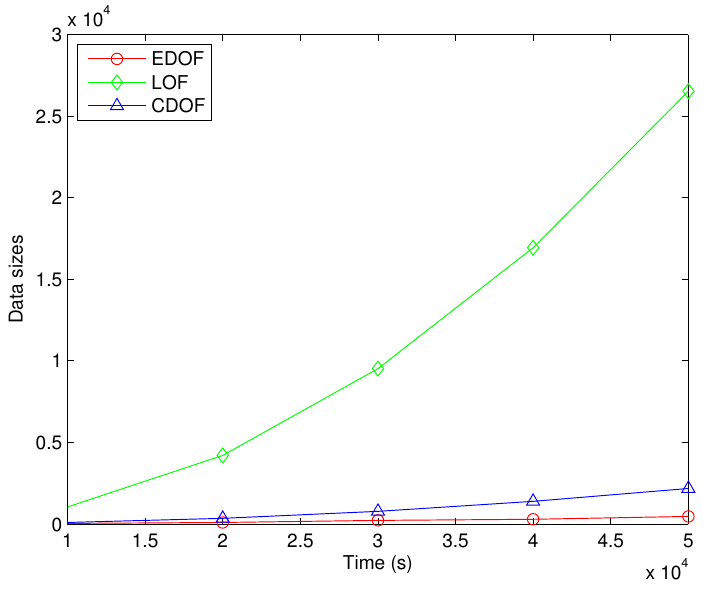
\includegraphics[width=0.7\textwidth]{algorithm/run-time}
            \caption{Execution time of approximate commute time method versus
                Euclidean distance and local outlier factor methods}
        \end{figure}

        \column{0.5\textwidth}
        \begin{figure}[H]
            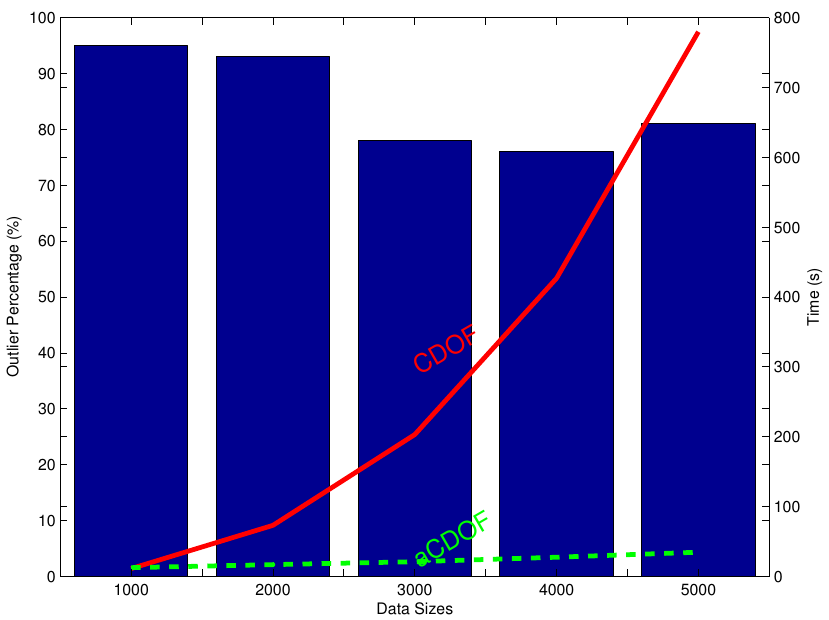
\includegraphics[width=0.7\textwidth]{algorithm/accuracy}
            \caption{Accuracy and execution time of approximated commute
                distance method compared to non-approximated method}
        \end{figure}
    \end{columns}

    \note<1>{These graphs show the measured performance of the chosen
        algorithm.}
    \note<2>{The left graph shows how run time (using \emph{approximated}
        commute time) is proportional to $O(n \log n)$, compared to:
        \begin{itemize}
            \item $O(n)$ using Euclidean distance
            \item $O(n^2)$ using local outlier factor
        \end{itemize}}
    \note<3>{The right graph shows how anomaly detection using
        \emph{approximated} commute time preserves a high percentage (84.6\% on
        average) of the top anomalies discovered without using approximations.}
\end{frame}

%%%%%%%%%%%%%%%%%%%%%%%%%%%%%%%%%%%%%%%%%%%%%%%%%%%%%%%%%%%%%%%%%%%%%%%%%%%%%%%%
% The Algorithm
%%%%%%%%%%%%%%%%%%%%%%%%%%%%%%%%%%%%%%%%%%%%%%%%%%%%%%%%%%%%%%%%%%%%%%%%%%%%%%%%
\subsection{The Algorithm}
\begin{frame}<1-2>[label=animation]{Animation}{A short animation illustrating the algorithm execution}
    \centering
    \movie[once,showcontrols]
        {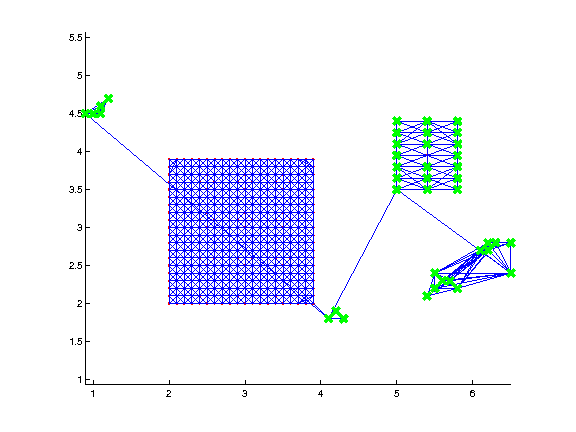
\includegraphics[width=0.8\textwidth]{pca/testoutrank}}
        {animation/testoutrank.avi}

    \note<1>{This slide shows a short animation, illustrating the execution of
        the chosen anomaly detection method on a data set of 441 2-dimensional
        vectors.

        In this animation, the yellow points indicate the current block that is
        being processed. Each vector within the block is compared to all other
        vectors in the data set, illustrated by the blue marker in the
        animation.

        Each vector in the current block is given a score, a monotonic
        decreasing function that provides a heuristic to estimate if any given
        vector may be an outlier.}

    \note<2>{The current `best' outliers are highlighted in green in the
        animation. As the algorithm processes further blocks of data, the set of
        current outliers converges to the final set of outliers.

        If the score for any vector in the current block becomes less than the
        lowest score from the set of current outliers, then this vector is no
        longer considered to be a possible outlier, and is pruned from the data
        set. The pruned vectors appear in red in the animation.}
\end{frame}
